\documentclass[aspectratio=169,t,xcolor=table]{beamer}
\usepackage[utf8]{inputenc}

\usepackage{booktabs} 
\usepackage{subcaption}
\usepackage{epigraph}
\usepackage[outercaption]{sidecap}    
\usepackage{tikz}


\usetheme{Ufg}

%-------------------------------------theorems--------------
\newtheorem{conj}{Conjetura}
\newtheorem{defi}{Definition}
\newtheorem{teo}{Teorema}
\newtheorem{lema}{Lema}
\newtheorem{prop}{Proposição}
\newtheorem{cor}{Corolário}
\newtheorem{ex}{Example}
\newtheorem{exer}{Exercício}

\setbeamertemplate{theorems}[numbered]
\setbeamertemplate{caption}[numbered]

%-------------------------------------------------------------%
%----------------------- Primary Definitions -----------------%

\definecolor{color1}{RGB}{0,0,90} % Color of the article title and sections
\definecolor{color2}{RGB}{0,20,20} % Color of the boxes behind the abstract and headings
\definecolor{keys1}{rgb}{0.0, 0.29, 0.33}
\definecolor{keys2}{rgb}{0.25, 0.7, 0.55}
\definecolor{keys3}{rgb}{0.1, 0.3, 0.4}
\definecolor{keys4}{rgb}{0.21, 0.46, 0.53}
\definecolor{strings}{rgb}{0.0, 0.47, 0.44}
\definecolor{comments}{rgb}{0.4, 0.4, 0.5}
\definecolor{terminaltext}{rgb}{1,1,1}
\definecolor{terminalbackground}{rgb}{0.2,0.2,0.25}

\usepackage{listings}

\lstset{
  xleftmargin=8pt,
  xrightmargin=0pt,
  framexleftmargin=0pt,
  framexrightmargin=0pt,
  basicstyle={\fontsize{8pt}{10pt}\ttfamily},
  columns=flexible,
  keepspaces=false,
  showstringspaces=false,
  commentstyle= \color{comments},
  stringstyle= \color{strings},
  breaklines=false,
  postbreak=\mbox{$\hookrightarrow$\space}
}

\lstdefinelanguage{Terminal}{
  framexleftmargin=3pt,
  framexrightmargin=3pt,
  framextopmargin=3pt,
  framexbottommargin=3pt,
  backgroundcolor=\color{terminalbackground},
  basicstyle={\fontsize{8pt}{10pt}\ttfamily\color{terminaltext}},
}

%%% Bibliography
\usepackage[style=numeric,backend=biber]{biblatex}
\addbibresource{thud.bib}


% This command set the default Color, is also possible to choose a custom color
\setPrimaryColor{UFGBlue} 

% First one is logo in title slide (we recommend use a horizontal image), and second one is the logo used in the remaining slides (we recommend use a square image)
\setLogos{lib/logos/infw.png}{lib/logos/infw2.png} 

% -------------------------------------- Title Slide Information
\begin{document}
\title[Inf UFG]{MONID}
\subtitle{A Temporal Logic Based Framework for Intrusion Detection}

\author{Zanolin Lorenzo\inst{1}}

\institute[UFG] % (optional)
{
  \inst{1}%
  DMIF\\
  University of Udine
}
\date{September 2023}
%-----------------------The next statement creates the title page.
\frame[noframenumbering]{\titlepage}

%------------------------------------------------Slide 1
\setLayout{vertical} % This command define the layout. 'vertical' can be replace with 'horizontal', 'blank, 'mainpoint', 'titlepage'

\begin{frame}
    \frametitle{Table of Contents}
    \tableofcontents
\end{frame}
%---------------------------------------------------------

\section{Introduction}

\setLayout{mainpoint}
\setBGColor{DarkPurple}
\begin{frame}{}
    \frametitle{Introduction}
\end{frame}
\setLayout{vertical}

\begin{frame}
    \frametitle{Intrusion Detection}
    \textit{Intrusion detection} means maintaining constant surveillance on a system in order to detect any misuse of these weak areas as soon as feasible so that they can be repaired.\\
    \vspace{5mm}
    There are three approaches:
    \begin{itemize}
        \item \textit{signature-based}: aims to identify patterns and match them with known signs of intrusions;
        \item \textit{anomaly-based}: can identify new attacks when it detects behavior that differs significantly from previously learned normal behavior;
        \item \textit{hybrid}: combines the best of both worlds by looking at patterns and one-off events.
    \end{itemize}
    \vspace{5mm}
    We will present MONID which is a \textit{signature-based} intrusion detector.
\end{frame}

\begin{frame}[allowframebreaks]{What is MONID?}
    MONID is a prototype which can detect intrusions on a system and operates in both online and offline modes.\\
    \vspace{5mm}
    In order:
    \begin{enumerate}
        \item we will use the logic \textbf{EAGLE} to define intrusion patterns using temporal logic formula $\varphi$; in this case the monitored formula will be $\psi=\square (\neg\varphi)$.
        \item MONID will create a stream of events $\sigma=\alpha_{1},\alpha_{2},\ldots$ obtained from a merge of the logs by ascending time order;
        \item a monitor will processes each event $\alpha_i$ as it happens and updates the monitored formula $\psi$ to store a relevant summary;
        \item an intrusion alarm is triggered if, for any reason, $\alpha_{1},\alpha_{2} \ldots\not\models\psi$.
    \end{enumerate}

    The architecture is the following.\\
    \vspace{2.5mm}
    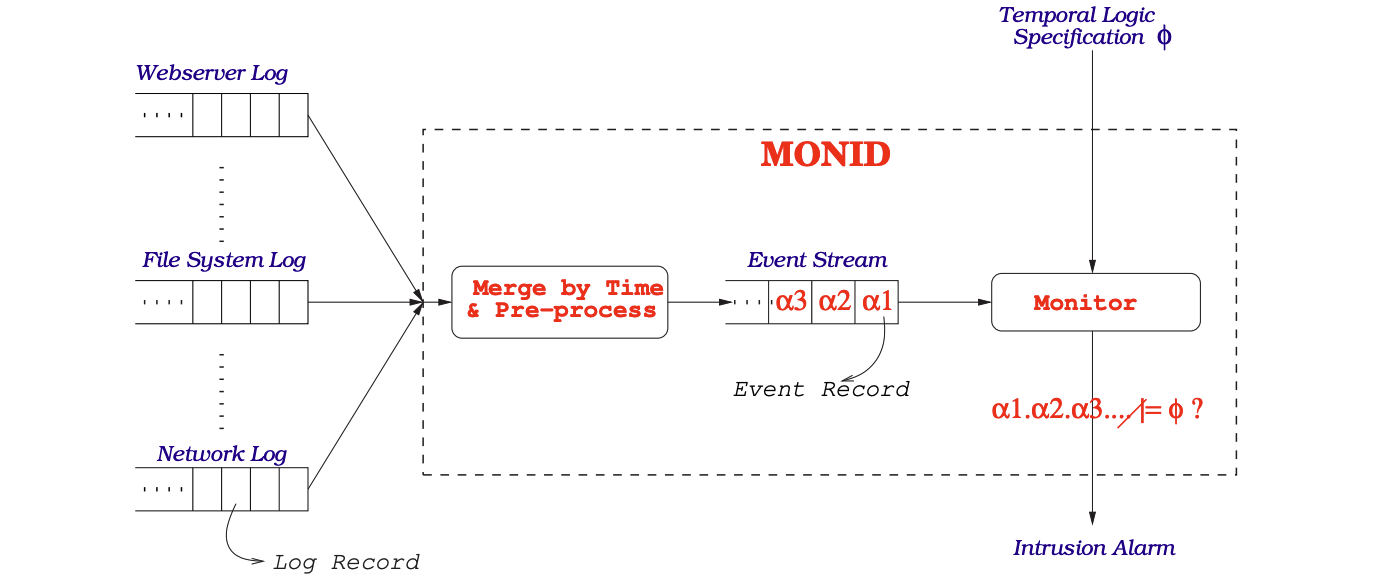
\includegraphics[scale=0.25]{images/monid.png}
\end{frame}

\begin{frame}
    \frametitle{Assumptions}
    Two assumptions must be made:

    \vspace{5mm}
    \begin{enumerate}
        \item There is a finite sequence of events called $\sigma=\alpha_{1},\ldots ,\alpha_{n}$ that is a merge of the system registered logs organized by ascending time. 
        The structure of an event record $\alpha_i$ is the following:
        \begin{align*}
            & \mathtt{LoginLogoutEvent}\{userId:\underline{\text{string}},\ action: \underline{\text{int}},\ time: \underline{\text{double}}\} 
        \end{align*}
        An example of event could be:\\ $\quad\quad\{userId:\mathtt{"Lori"},\ action:\mathtt{login},\ time:\mathtt{20}\}$
        \item For each attack, there is a formula $\psi$ which specifies the absence of it.
    \end{enumerate}
    \vspace{5mm}
    Now let us start on the basics of EAGLE.
\end{frame}


\section{EAGLE}

\setLayout{mainpoint}
\setBGColor{Ocean}
\begin{frame}{}
    \frametitle{EAGLE,\\ a Temporal Monitoring Logic}
\end{frame}
\setLayout{vertical}

\begin{frame}[allowframebreaks]{Basics}
    EAGLE offers a succinct but powerful set of primitives, supporting recursive parameterized equations with a minimal/maximal fix-point semantics together with three temporal operators: next-time ($\bigcirc$), previous-time ($\odot$), and concatenation ($\cdot$).\\
    \vspace{2.5mm}
    As a result, rules in EAGLE give us the power to create specific temporal operators as well as to bind and modify data. This property turns out to be crucial for succinctly expressing executions of attack-safe systems.\\
    \vspace{2.5mm}
    EAGLE operates with \textit{finite trace} semantics, meaning it checks formula satisfaction only at the end of a trace. However, in intrusion detection where event sequences can be infinite, the goal is to trigger an alarm as soon as a property is violated, thus MONID continuously checks the formula's satisfaction status after each event.\\
    \vspace{2.5mm}
    
    Let us start with an example.
    \begin{ex} 
    We want to express the property "\textit{Whenever there is a login by any user x, then eventually the user x logs out}". In EAGLE we can do it with the following rules:\\
    \vspace{2.5mm}
    $\quad \underline{\text{min}}\ \mathtt{EvLogout}(\underline{\text{string}}\ k) = (action = \mathtt{logout}\land userId = k) \lor \bigcirc \mathtt{EvLogout}(k) $\\
    $\quad \underline{\text{mon}}\ M_2 = ((action = \mathtt{login})\rightarrow \mathtt{EvLogout}(userId)) $\\
    \vspace{2.5mm}
    Once the rules are created, the monitor will evaluate and update the monitored formula $M_2$. 
    A possibile trace $\sigma=\alpha_1,\alpha_2 $ , where:\\
    \vspace{2.5mm} 
    $\alpha_1=\{userId:\mathtt{"Lori"},\ action:\mathtt{login},\ time:\mathtt{17.0}\}$ \\$\alpha_2=\{userId:\mathtt{"Lori"},\ action:\mathtt{logout},\ time:\mathtt{150.0}\}$\\ 
    \vspace{2.5mm}
    satisfies $M_2$.
    \end{ex}
\end{frame}

\begin{frame}[allowframebreaks]{Syntax}
    Each specification $S$ is made up of an observer part $O$ and a declaration part $D$.
    \begin{align*}
    S &::= D \, O \\
    D &::= R^* \\
    O &::= M^* \\
    R &::= \{\underline{\text{max}}\ |\ \underline{\text{min}} \}\ N(T_1\ x_1, \ldots, T_n\ x_n) = F \\
    M &::= \underline{\text{mon}}\ N = F \\
    T &::= \underline{\text{Form}}\ |\ \text{primitive type} \\
    F &::= \text{expression}\ |\ \underline{\text{true}}\ |\ \underline{\text{false}}\ |\ \neg F\ |\ F_1 \land F_2\ |\ F_1 \lor F_2\ |\\
            &F_1 \rightarrow F_2\ |\ \bigcirc F\ |\ \odot F\ |\ F_1 \cdot F_2\ |\ N(F_1, \ldots, F_n)\ |\ x_i
    \end{align*}
    Let us focus on some details.\\
    Definitions can start with different keywords:
    \begin{itemize}
        \item $\underline{\text{mon}}$: specifies the EAGLE formulas to be monitored and cannot have a recursive definition; as already told, these kind of rules will evolve as new events appear.
        \item $\underline{\text{max}}$: defines \textit{safety properties} (nothing bad ever happens) and have a maximal interpretation.
        \item $\underline{\text{min}}$: defines \textit{liveness properties} (something good eventually happens) and have a minimal interpretation.
    \end{itemize}

    \begin{block}{Note.}    
        The difference between maximal and minimal interpretation becomes important only when we are evaluating the at the boundaries of a trace: $\underline{\text{max}}$ rules evaluates at $\underline{\text{true}}$ at initial and final istants, while $\underline{\text{min}}$ rules evaluates at $\underline{\text{false}}$.
    \end{block}    
    \newpage
    To better understand the mechanism, let us introduce an example.\\ Given the definition 
    \begin{align*}
        & \underline{\text{min}}\ \mathtt{Property}(\underline{\text{Form}}\ F) =F \lor \bigcirc \mathtt{Property}(F)
    \end{align*} 
    and the sequence $\sigma=\alpha_{1},\ldots ,\alpha_{n}$, $\mathtt{Property}$ will evaluate to \textit{true} 
    \begin{align*}
        & evaluate(\ldots evaluate(evaluate(\mathtt{Property},\alpha_1),\alpha_2),\ldots,\alpha_n)=true
    \end{align*}
    if and only if the rule is true at some given event $\alpha_i$. Once the sequence has been completely analyzed, we will obtain the following big disjunction: 
    \begin{align*}
        & F \lor \bigcirc(F \lor \bigcirc(\ldots F \lor \bigcirc \mathbf{Property(F)})) 
    \end{align*}
    $\mathbf{Property(F)}$ will be evaluated as false since it is the last of a big disjunction and we want to close it.

\end{frame}

\begin{frame}[allowframebreaks]{Semantics}
    The semantics of the logic is defined in terms of the \textit{satisfaction} relation $\models$ which defines whether a finite execution trace $\sigma$ satisfies the specification $\varphi=D \, O$.\\
    \vspace*{5mm}
    Given a trace $\sigma$ and a specification $D \, O$, satisfaction is defined as follows:
    \[
    \sigma \models D \, O \text{ iff } \forall (\underline{\text{mon}}\ N = F) \in O.\ \sigma ,1 \models_D \, F
    \]
    In other words, a trace satisfies a specification if it fulfills each monitored formula ($\underline{\text{mon}}$) when monitoring from position 1, which is the initial state.\\
    \vspace*{5mm}
    In the following slide we will present the definition of the satisfaction relation $\models_D \subseteq (Trace \times \mathbb{N}) \times \underline{\text{Form}}$ for a set of rule definitions $D$. 
    
    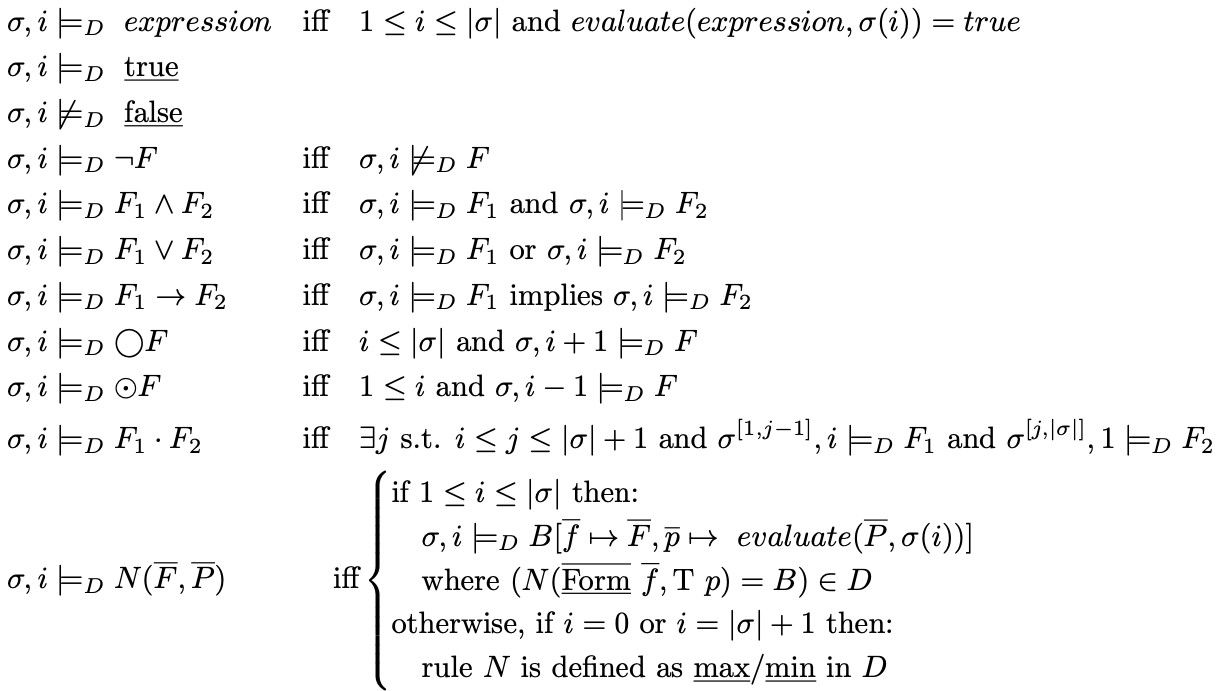
\includegraphics[scale=0.27]{images/semantics.png}
\end{frame}

\begin{frame}[allowframebreaks]{Evaluation algorithm}
    As we can see, a function called $evaluate$ emerges; there are additional functions as well. Let us list them.
    \begin{itemize}
        \item $evaluate: \underline{\text{Form}} \times \underline{\text{State}}$. This function is used to evolve at every event the monitored formulas.
        \item $update: \underline{\text{Form}} \times \underline{\text{State}} \to \underline{\text{Form}}$. This function is used by $evaluate$ to pre-evaluate a formula if it is guarded by the previous operator $\odot$
        \item $value : \underline{\text{Form}} \rightarrow \{ \underline{\text{true}}, \underline{\text{false}} \}$. This function returns true if and only if $\sigma,|\sigma|+1 \models F$ (or $\sigma,0 \models F$), and returns false otherwise.
    \end{itemize}
    \begin{block}{Note.}
        Formally, a formula $F' = evaluate(F, \alpha_i)$ is created when a formula $F$ is evaluated at an event $\alpha_i = \sigma(i)$ and has the condition that $\sigma, i \models F$ if and only if $\sigma, i+1 \models F'$. With $F$ being the evolved formula, we compute the boolean function $value(F)$ at the conclusion of the trace.
    \end{block}

    \newpage
    More details are in the paper; let us introduce an example.
    \begin{ex}
        Given the following rules\\
        \vspace{1.5mm}
        $\quad\underline{\text{max}}\ \mathtt{Always}(\underline{\text{Form}}\ F)  = F \land \bigcirc \mathtt{Always}(F)$ \\
        $\quad\underline{\text{min}}\ \mathtt{EvTimedLogout}(\underline{\text{string }} k, \underline{\text{double }} t, \underline{\text{double }} \delta) = (\text{time} - t \leq \delta)$ \\
        $\quad\quad\quad\quad\quad \land ((action = \mathtt{logout} \land userId = k) \lor \bigcirc \mathtt{EvTimedLogout}(k, t, \delta))$ \\
        $\quad\underline{\text{mon}}\ M_3  = \mathtt{Always}((action = \mathtt{login}) \rightarrow \mathtt{EvTimedLogout}(userId,time, 100))$ \\
        \vspace{1.5mm}
        and a trace $\sigma=\alpha_1,\alpha_2$ , where\\\vspace{1.5mm} $\quad\alpha_1=\{userId:\mathtt{"Lori"},\ action:\mathtt{login},\ time:\mathtt{17.0}\}$\\ $\quad\alpha_2=\{userId:\mathtt{"Lori"},\ action:\mathtt{logout},\ time:\mathtt{150.0}\}$.\\ \vspace{1.5mm}$M_3$ gets modified, at first step, in \\
        \vspace{1.5mm}
        $\quad evaluate(M_3,\alpha_1)  = \mathtt{EvTimedLogout("Lori",17.0, 100)}$ \\ 
        $\quad\quad\quad\quad\quad \land\ \mathtt{Always}((action = \mathtt{login}) \rightarrow \mathtt{EvTimedLogout}(userId,time, 100))$.
    \end{ex}    %continuazione?
\end{frame}

\begin{frame}{Relationship with LTL+P}
    We can define both \textbf{Future Time LTL} and \textbf{Past Time LTL} operators. As example, let us show the future ones.
    \begin{align*}
        & \underline{\text{min}}\ \mathtt{Next}(\underline{\text{Form}}\ F) = \bigcirc F \\
        & \underline{\text{max}}\ \mathtt{Always}(\underline{\text{Form}}\ F) = F \land \bigcirc \mathtt{Always}(F) \\
        & \underline{\text{min}}\ \mathtt{Eventually}(\underline{\text{Form}}\ F) = F \lor \bigcirc \mathtt{Eventually}(F) \\
        & \underline{\text{min}}\ \mathtt{Until}(\underline{\text{Form}}\ F_1, \underline{\text{Form}}\ F_2) = F_2 \lor (F_1 \land \bigcirc \mathtt{Until}(F_1,F_2))
    \end{align*}
    By combining the definitions for the future and past time LTL as defined above, we obtain a temporal logic over the future, present and past, in which one can freely intermix the future and past time modalities;\\thus, we can state that EAGLE is expressive at least as LTL+P.

\end{frame}

\section{Attacks detection}
\setLayout{mainpoint}
\setBGColor{LightOrange}
\begin{frame}{}
    \frametitle{Attacks detection}
\end{frame}
\setLayout{vertical}

\begin{frame}
    \frametitle{Smurf Attacks}
    A \textit{smurf attack} is a DDoS attack targeting computer networks by sending large volumes of ICMP echo request packets to a broadcast address. The attacker spoofs the source IP address to make it appear as originating from the victim's IP address, causing all devices to respond with ICMP echo replies.\\
    \vspace{2.5mm}
    In this example we will use \textit{tcpdump} to obtain the logs from the network interface; the formula that describes the absence of the attack is the following:
    \begin{align*}
        & \underline{\text{max}}\ \mathtt{SmurfAttack()} = (type = \text{"ICMP"})\land isBroadcast(ip) \\
        & \underline{\text{mon}}\ \mathtt{SmurfSafety} =\ \mathtt{Always}(\neg\ \mathtt{SmurfAttack()}) 
    \end{align*}
    where \textit{isBroadcast}() checks whether the destination’s IP address is a broadcast ip, i.e. all the host bits are set to 1.
\end{frame}

\begin{frame}
    \frametitle{Cookie-stealing Attacks}
    A \textit{cookie} is a technique used by web application servers to track client-specific session data; these tools are automatically included in client requests. When a malicious user uses an old cookie provided to a different IP address to take over a session, it is considered an attack.\\ \vspace{2.5mm} At this point we need to look at web-server log; the formula that describes the absence of the attack is the following:
    \begin{align*}
        & \underline{\text{min}}\ \mathtt{Hijack}(\underline{\text{string}}\ c,\underline{\text{string}}\ i) = ((name=c)\land\neg(ip=i))\lor\odot\ \mathtt{Hijack}(c,i) \\
        & \underline{\text{mon}}\ \mathtt{CookieSafe} =\ \mathtt{Always}(\neg\mathtt{Hijack}(name,ip)) 
    \end{align*}
    where a single cookie is identified from $c$ and it can be associated only at a single $ip$.
\end{frame}

\begin{frame}
    \frametitle{Multi-domain Buffer Overflows attacks}
    A \textit{buffer overflow} attack uses memory manipulation to overflow a buffer, modifying an address to point to malicious code. Data from network and web server access logs are analyzed to determine when the attack occurred and if no matching log record is found within a timeout, the attack is successful. To capture this scenario we use the following formulas:
    \begin{align*}
        & \underline{\text{min}}\ \mathtt{EventuallyClosed}(\underline{\text{long}}\ t,\underline{\text{long}}\ d,\underline{\text{string}}\ i1,\underline{\text{string}}\ i2) = (time-t<d)\\
        & \quad\quad\land ((ip1=i1\land ip2=i2\land log=web\land type=closed)\\
        & \quad\quad\quad\lor \bigcirc\mathtt{EventuallyClosed}(t,d,i1,i2) ) \\
        & \underline{\text{mon}}\ \mathtt{BufferSafe} =\ \mathtt{Always}((log=network\land type=binary) \\
        & \quad\quad\rightarrow\mathtt{EventuallyClosed}(time,100,ip1,ip2))
    \end{align*}
    where a session, identified by $(ip1,ip2)$, must end within $100$ seconds if there is a $binary$ access.
\end{frame}

\begin{frame}
    \frametitle{Password guessing attacks}
    If the system accepts telnet connections for remote login, an attacker can easily compromise a user's password by guessing multiple passwords for a specific user name. We can detect with the following:
    \begin{align*}
        & \underline{\text{max}}\ \mathtt{Failure}() = (type=login)\land \neg success\\
        & \underline{\text{max}}\ \mathtt{Guess}(\underline{\text{string}}\ i) = (ip=i)\land \mathtt{Failure}()\\
        & \underline{\text{max}}\ \mathtt{Counter}(\underline{\text{long}}\ t, \underline{\text{long}}\ d, \underline{\text{int}}\ c,\underline{\text{string}}\ i,\underline{\text{int}}\ C) = (time-t<d)\\
        & \quad\quad\rightarrow((\mathtt{Guess}(i)\rightarrow(c\leq C\land \bigcirc\mathtt{Counter}(t,d,c+1,i,C)))  \\
        & \quad\quad\land(\neg \mathtt{Guess}(i)\rightarrow\mathtt{Counter}(t,d,c,i,C))) \\
        & \underline{\text{mon}}\ \mathtt{PassGuessSafe} =\ \mathtt{Always}(\mathtt{Failure}()\rightarrow\mathtt{Counter}(time,300,1,ip,3)) 
    \end{align*}
    where an attacks is detected if a password has been incorrectly guessed for $3$ times within $300$ seconds.
\end{frame}

\begin{frame}
    \frametitle{Port Scanning attacks}
    \textit{Port scanning} is a method used to identify exploitable communication channels in networks; it involves probing network ports and keeping useful information for attacks. The victim machine suspect port scans as malicious when the counter of reached ports exceeds a specific threshold. The formulas are the following:
    \begin{align*}
        & \underline{\text{max}}\ \mathtt{NewPort}(\underline{\text{string}}\ i1,\underline{\text{string}}\ i2,\underline{\text{Set}}\ S) = (i1=ip1)\land(i2=ip2)\land (port \notin S)\\
        & \underline{\text{max}}\ \mathtt{Counter}(\underline{\text{long}}\ t, \underline{\text{long}}\ d, \underline{\text{int}}\ c,\underline{\text{string}}\ i1,\underline{\text{string}}\ i2,\underline{\text{Set}}\ S,\underline{\text{int}}\ C) = (time-t<d)\\
        & \quad\quad\rightarrow((\mathtt{NewPort}(i1,i2,S)\rightarrow(c\leq C\land \bigcirc\mathtt{Counter}(t,d,c+1,i1,i2,S\cup\{port\},C)))  \\
        & \quad\quad\land(\neg \mathtt{NewPort}(i1,i2,S)\rightarrow\mathtt{Counter}(t,d,c,i1,i2,S,C))) \\
        & \underline{\text{mon}}\ \mathtt{PortScanSafe} =\ \mathtt{Always}(\mathtt{Counter}(time,100,1,ip1,ip2,\{port\},10)) 
    \end{align*}
    where we checks if the number of (new) port scans between $ip1,ip2$ does not exceed a threshold of $10$ within $100$ seconds.
\end{frame}

\begin{frame}
    \frametitle{Performances}
    MONID was evaluated against smurf, port-sweep, and password-guessing attacks using DARPA Intrusion Detection Evaluation dataset in offline mode, detecting 5 password-guess attacks and 2 port-sweep attacks.
    \begin{figure}[!htb]
        \begin{center}
            \begin{minipage}{0.45\textwidth}
                \centering
                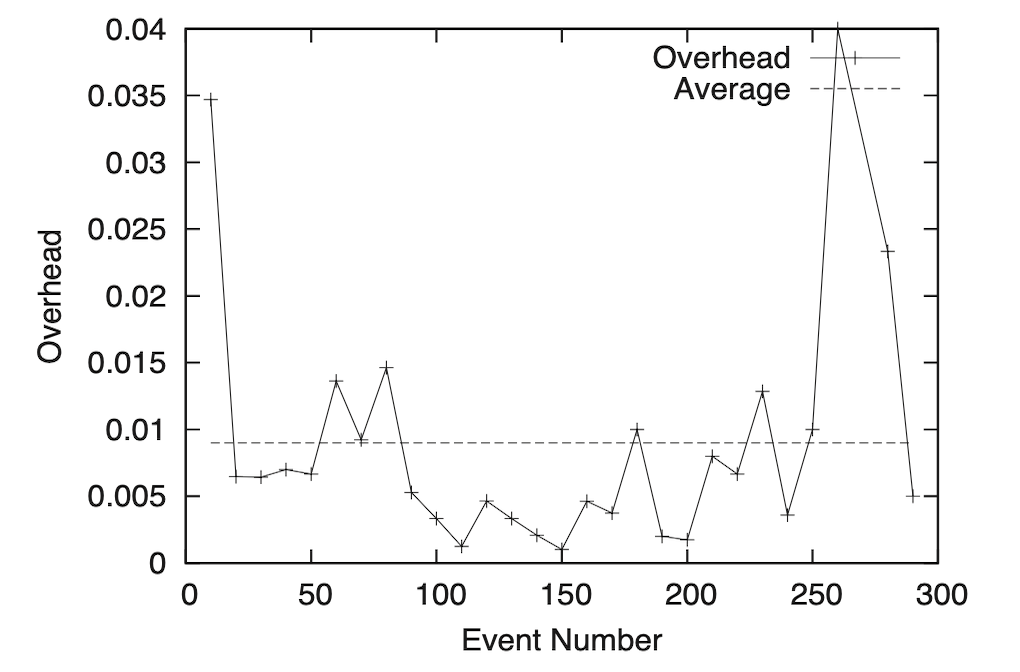
\includegraphics[width=\linewidth]{images/graph 1.png}
                \caption{Performances overhead of Port-Sweep attacks.}\label{graph1}
            \end{minipage}
            \hfill
            \begin{minipage}{0.45\textwidth}
                \centering
                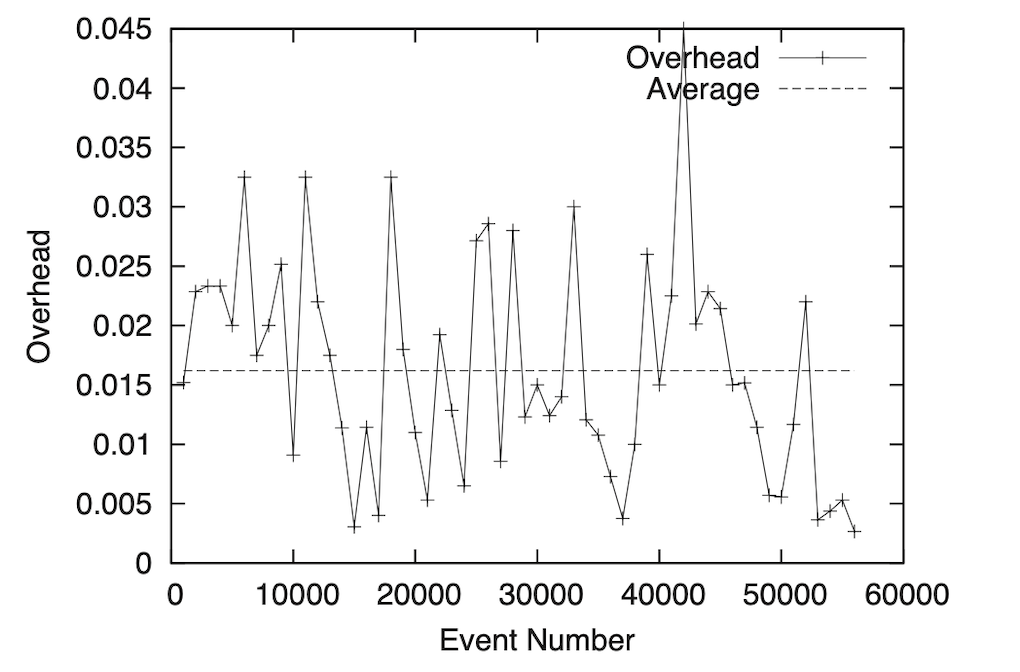
\includegraphics[width=\linewidth]{images/graph 2.png}
                \caption{Performances overhead of Password-Guessing attacks.}\label{graph2}
            \end{minipage}
        \end{center}
    \end{figure}

\end{frame}

\section{Conclusions}
\setLayout{mainpoint}
\setBGColor{LightGray}
\begin{frame}{}
    \frametitle{Conclusions}
\end{frame}
\setLayout{vertical}


\begin{frame}
    \frametitle{Conclusions}
    In conclusion:
    \begin{itemize}
        \item We have introduced the MONID framework and explained how it works.
        \item We then proceeded introducing a new temporal logic named EAGLE, which serves as the foundation for the MONID framework.
        \item We have presented some example of formulas which aims at recognize some attacks patterns.
    \end{itemize}
    \vspace{2.5mm}
    Due to the little overhead involved in the computation and the great performances of MONID when utilized offline, we can state that this method should still be useful in theory today. 
    
    \vspace{2.5mm}
    Attacks nowadays become more and more complex but once a pattern is found, we can represent it with EAGLE.
\end{frame}

\begin{frame}[allowframebreaks]{References}
    \nocite{*} 
    \printbibliography
\end{frame}

\setLayout{mainpoint}
\setBGColor{DarkGray}
\begin{frame}{}
    \frametitle{Thanks for the attention}
\end{frame}
\setLayout{vertical}

\end{document}